% WingJEPA poster, 48 x 36 in (landscape). Compile: tectonic -X compile poster.tex
\documentclass{article}
\usepackage[paperwidth=48in,paperheight=36in,margin=0.8in]{geometry}
\usepackage[T1]{fontenc}
\usepackage{lmodern}
\usepackage[scaled=0.95]{helvet}
\renewcommand{\familydefault}{\sfdefault}
\usepackage{amsmath,amssymb}
\usepackage{exscale}
\hyphenation{SIGReg SkyJEPA McNemar Direct physics Predictive frozen}
\usepackage{xcolor}
\usepackage{graphicx}
\usepackage{tikz}
\usepackage[most]{tcolorbox}
\usepackage{array,booktabs}
\usepackage{enumitem}
\usepackage{url}
\usepackage{ragged2e}
\usepackage{multicol}
\usetikzlibrary{calc}

\pagestyle{empty}
\setlength{\parindent}{0pt}
\setlength{\parskip}{0.28em}
\graphicspath{{figures/}}

% ---------------------------------------------------------------- colors
\definecolor{navy}{HTML}{1F3A5F}
\definecolor{direct}{HTML}{2E6DB4}
\definecolor{jepa}{HTML}{E07B1A}
\definecolor{phys}{HTML}{2E8B57}
\definecolor{txt}{HTML}{333333}
\definecolor{soft}{HTML}{6B6B6B}
\definecolor{pagebg}{HTML}{F3F5F8}
\color{txt}

% ---------------------------------------------------------------- font sizes
\renewcommand{\normalsize}{\fontsize{25}{30}\selectfont
  \abovedisplayskip 6pt plus 2pt \belowdisplayskip 6pt plus 2pt
  \abovedisplayshortskip 3pt \belowdisplayshortskip 5pt}
\renewcommand{\small}{\fontsize{22.5}{27}\selectfont}
\renewcommand{\footnotesize}{\fontsize{20.5}{24.5}\selectfont}
\renewcommand{\large}{\fontsize{32}{39}\selectfont}
\renewcommand{\Large}{\fontsize{40}{47}\selectfont}
\normalsize

% ---------------------------------------------------------------- helpers
\newcommand{\Dir}[1]{\textcolor{direct}{\textbf{#1}}}
\newcommand{\Jep}[1]{\textcolor{jepa}{\textbf{#1}}}
\newcommand{\Phy}[1]{\textcolor{phys}{\textbf{#1}}}
% model names (same short names as the figures)
\newcommand{\mPred}{\Dir{Predictive (one-step)}}
\newcommand{\mDM}{\Dir{Direct + MLP}}
\newcommand{\mJM}{\Jep{JEPA + MLP}}
\newcommand{\mJP}{\Jep{JEPA} \Phy{+ physics}}
\newcommand{\mDFP}{\Dir{Direct frozen} \Phy{+ physics}}
\newcommand{\mDPE}{\Dir{Direct} \Phy{+ physics} \textbf{(end to end)}}
\newcommand{\mMLP}{\textbf{Plain MLP}}
\newcommand{\mTECS}{\textbf{TECS}}
\newcommand{\cnum}[1]{\tikz[baseline=(c.base)]\node[circle,fill=white,text=navy,
  inner sep=0pt,minimum size=1.25em,font=\bfseries](c){#1};}
\renewcommand{\cite}[1]{\textcolor{soft}{[#1]}}

\setlist{nosep,leftmargin=1.0em,labelsep=0.4em,topsep=0.1em,itemsep=0.14em}
\setlist[itemize,1]{label=\textcolor{navy}{\raisebox{0.12em}{\scalebox{0.8}{$\blacktriangleright$}}}}

% figure with a fixed bounding box: picks the file up when it exists
\newcommand{\fig}[3]{% {file}{width}{max height}
  \par\vspace{0.2em}{\centering
  \IfFileExists{figures/#1}{\includegraphics[width=#2,height=#3,keepaspectratio]{#1}}%
  {\fcolorbox{soft}{white}{\parbox[c][#3][c]{\dimexpr#2-2\fboxsep-2\fboxrule\relax}{\centering
     \textcolor{soft}{placeholder: \texttt{figures/#1}}}}}\par}\vspace{0.2em}}
\newcommand{\figcap}[1]{{\footnotesize\textcolor{soft}{#1}\par}\vspace{0.25em}}

% ---------------------------------------------------------------- boxes
\newtcolorbox{panel}[3][]{enhanced, arc=6pt, boxrule=1.5pt, colframe=navy!35,
  colback=white, before upper={\RaggedRight}, left=0.27in, right=0.27in, top=0.18in, bottom=0.18in,
  toptitle=0.11in, bottomtitle=0.11in,
  colbacktitle=navy, coltitle=white, fonttitle=\Large\bfseries,
  title={\RaggedRight\cnum{#2}\hspace{0.35em}#3}, before skip=0pt, after skip=0pt, valign=top, #1}

\newtcolorbox{keybox}[1][]{enhanced, arc=4pt, boxrule=1.2pt, colframe=#1, colback=#1!7,
  before upper={\RaggedRight}, left=0.18in, right=0.18in, top=0.1in, bottom=0.1in,
  before skip=0.3em, after skip=0.3em}
\newtcolorbox{progbox}{enhanced, arc=4pt, colback=gray!6, frame hidden,
  borderline={1.6pt}{0pt}{soft,dashed}, before upper={\RaggedRight},
  left=0.18in, right=0.18in, top=0.1in, bottom=0.1in, before skip=0.4em, after skip=0pt}

% ---------------------------------------------------------------- columns
% every column has the same height; the last panel of a column fills it
\newlength{\colH}\setlength{\colH}{28.75in}
\newlength{\gapV}\setlength{\gapV}{0.3in}
\newlength{\cw}\setlength{\cw}{9.07in}
\newlength{\colgap}\setlength{\colgap}{\dimexpr(\textwidth-5\cw)/4\relax}
\newsavebox{\colabove}
\newlength{\restH}
\newlength{\curH}\setlength{\curH}{\colH}
\newlength{\refsH}\setlength{\refsH}{3.0in}
\newlength{\topH}
\newsavebox{\refsbox}
\newcommand{\fillrest}{\usebox{\colabove}\par\vspace{\gapV}%
  \setlength{\restH}{\dimexpr\curH-\ht\colabove-\dp\colabove-\gapV\relax}}

% ================================================================ document
\begin{document}

% background, header band, footer (full bleed)
\begin{tikzpicture}[remember picture, overlay]
  \fill[pagebg] (current page.south west) rectangle (current page.north east);
  \fill[navy] (current page.north west) rectangle ($(current page.north east)+(0,-4.55in)$);
  \fill[jepa] ($(current page.north west)+(0,-4.55in)$) rectangle ($(current page.north east)+(0,-4.68in)$);
  \node[anchor=base, font=\fontsize{24}{28}\selectfont, text=soft] at ($(current page.south)+(0,0.3in)$)
    {Code and results: \textcolor{navy}{\url{https://github.com/clementdumeril/WingJEPA}}};
\end{tikzpicture}%
\vspace*{-0.5in}
\begin{center}
  {\color{white}
  {\fontsize{88}{100}\selectfont\bfseries Does a JEPA world model help fly an unidentified fixed-wing aircraft?\par}
  \vspace{0.2in}
  {\fontsize{50}{60}\selectfont A controlled test of the SkyJEPA recipe on a simulated Ultra Stick 120\par}
  \vspace{0.16in}
  {\fontsize{40}{48}\selectfont \textbf{Clément Dumeril}\quad\textcolor{white!72!navy}{UC Berkeley, Physics-Inspired Machine Learning, Fall 2026}\par}}
\end{center}

\vspace{0.5in}
% ---------------------------------------------------------------- answer banner
\begin{tcolorbox}[enhanced, arc=8pt, boxrule=2.5pt, colframe=jepa, colback=jepa!8,
  left=0.45in, right=0.45in, top=0.13in, bottom=0.13in, before skip=0pt, after skip=0pt]
  \fontsize{33}{40}\selectfont
  \begin{tabular}{@{}m{5.6in}@{\hspace{0.4in}}m{38.4in}@{}}
  \textcolor{jepa}{\bfseries Answer in one line} &
  \textbf{In this setting, no.} On a fixed wing whose commands are not forces, \mJP{} reproduces SkyJEPA's
  ranking on training-range aircraft, but the two controls SkyJEPA did not run predict better
  (the same \Phy{physics head} trained end to end, and a \mMLP{} of 10.6k parameters),
  and the \Jep{JEPA} latent keeps little motor or CG information.
  \end{tabular}
\end{tcolorbox}

\vspace{0.33in}
% ================================================================ columns
\noindent
% ---------------------------------------------------------------- columns 1-2 + references
\sbox{\refsbox}{\begin{minipage}{\dimexpr2\cw+\colgap\relax}
\begin{tcolorbox}[enhanced, arc=6pt, boxrule=1.5pt, colframe=navy!35, colback=white,
  left=0.27in, right=0.27in, top=0.12in, bottom=0.12in, before skip=0pt, after skip=0pt,
  before upper={\RaggedRight}]
{\fontsize{19}{22.5}\selectfont\setlength{\columnsep}{0.4in}
\begin{multicols}{2}
\raggedcolumns
\textbf{References}\vspace{-0.1em}
\begin{enumerate}[label={[\arabic*]},leftmargin=1.75em,itemsep=0.02em]
\item Rao et al., SkyJEPA, arXiv:2606.23444v2, 2026.
  \item Balestriero \& LeCun, LeJEPA, arXiv:2511.08544, 2025.
  \item LeCun, A Path Towards Autonomous Machine Intelligence, 2022.
  \item Williams et al., Information theoretic MPC for model-based RL, ICRA 2017.
  \item Littwin et al., How JEPA avoids noisy features: the implicit bias of deep linear self distillation networks, NeurIPS 2024.
  \item Kumar et al., RMA, RSS 2021.
  \item Nagabandi et al., Neural network dynamics for model-based deep RL with model-free fine-tuning, ICRA 2018.
  \item UMN UAV Research Group, UMNUAV\_sim\_v4 (BSD), with NASA Langley wind-tunnel data.
  \item Hovakimyan \& Cao, L1 Adaptive Control Theory, SIAM, 2010.
  \item Smeur, Chu \& de Croon, Adaptive incremental nonlinear dynamic inversion for attitude control of micro air vehicles, J.\ Guidance, Control, and Dynamics, 2016.
  \item O'Connell et al., Neural-Fly enables rapid learning for agile flight in strong winds, Science Robotics, 2022.
  \item Lambregts, Vertical flight path and speed control autopilot design using total energy principles, AIAA, 1983.
\end{enumerate}
\end{multicols}\par}
\end{tcolorbox}
\end{minipage}}%
\setlength{\refsH}{\dimexpr\ht\refsbox+\dp\refsbox\relax}%
\setlength{\topH}{\dimexpr\colH-\refsH-\gapV\relax}%
\setlength{\curH}{\topH}%
\begin{minipage}[t][\colH][t]{\dimexpr2\cw+\colgap\relax}\vspace{0pt}
% ---------------------------------------------------------------- column 1
\begin{minipage}[t][\topH][t]{\cw}\vspace{0pt}
\sbox{\colabove}{\begin{minipage}{\cw}
\begin{panel}{1}{The problem}
\textbf{Goal.} Fly a fixed-wing aircraft whose aerodynamics, motor and center of gravity are unknown
(new airframe, new payload or propeller) from its last measurements, with noisy sensors,
without an identification flight.

\textbf{What exists}
\begin{itemize}
  \item \textbf{System identification}: one dedicated test campaign per airframe, redone after every change.
  \item \textbf{Adaptive control} (L1 \cite{9}, INDI \cite{10}): adapts the controller but gives no
        multi-step model to plan with.
  \item \textbf{Learned adaptation}: RMA \cite{6} (policy trained with the true parameters),
        Neural-Fly \cite{11} (learned residual forces with online adaptation).
\end{itemize}
\textbf{Approach studied.} A learned \textbf{world model inside MPPI} \cite{4}, which predicts how the
current aircraft will move.
\end{panel}
\end{minipage}}%
\fillrest
\begin{panel}[height=\restH]{2}{What SkyJEPA claims, and what it did not test}
SkyJEPA \cite{1}: a JEPA world model \cite{3} of a quadrotor (TCN encoders, GRU predictor, SIGReg \cite{2})
plus a physics-informed prober, trained in simulation on randomized vehicles, used in MPPI.
\begin{itemize}
  \item Their Table III (horizon not stated): \Jep{JEPA} + \Phy{physics prober} \textbf{1.43\,m}, best;
        reconstruction + \Phy{physics prober} \textbf{1.53\,m}; \Jep{JEPA} + MLP prober \textbf{5.56\,m};
        Predictive \textbf{8.80\,m}.
  \item With the \Phy{physics prober}, JEPA adds only \textbf{0.10\,m} over reconstruction
        (1.43 vs 1.53\,m).
\end{itemize}
Their actions are the four motor forces, so the thrust is known from the action:
\[ \dot v = \frac{\displaystyle\sum\nolimits_i f_i}{m}\, R\, e_3 - g + \Delta \dot v \]
\textbf{Not tested}: a plain MLP, and the physics prober on a predictive (state-loss) model,
frozen or trained end to end.
\fig{fig_skyjepa_gap.pdf}{\linewidth}{4.8in}
\figcap{Position error divided by the one-step Predictive model (SkyJEPA: 8.80\,m; ours: 37.5\,m at
5\,s, training-range aircraft, mean of 3 seeds).}
\begin{keybox}[navy]
\hyphenpenalty=10000
\textbf{Q1}\enspace Does JEPA predict better?\\
\textbf{Q2}\enspace Does it identify the aircraft without labels?\\
\textbf{Q3}\enspace Is it less sensitive to sensor noise at equal training?\\
\textbf{Q4}\enspace Does it fly better in closed loop?
\end{keybox}
\end{panel}
\end{minipage}%
\hfill
% ---------------------------------------------------------------- column 2
\begin{minipage}[t][\topH][t]{\cw}\vspace{0pt}
\begin{panel}[height=\topH]{3}{Test bench}
\textbf{Simulator.} Python port of the University of Minnesota Ultra Stick 120 6-DoF model \cite{8}
(NASA wind-tunnel tables), checked against the reference trajectories.
\IfFileExists{../docs/figures/validation/ultrastick120_6dof_doublets.png}{%
  \par\vspace{0.15em}{\centering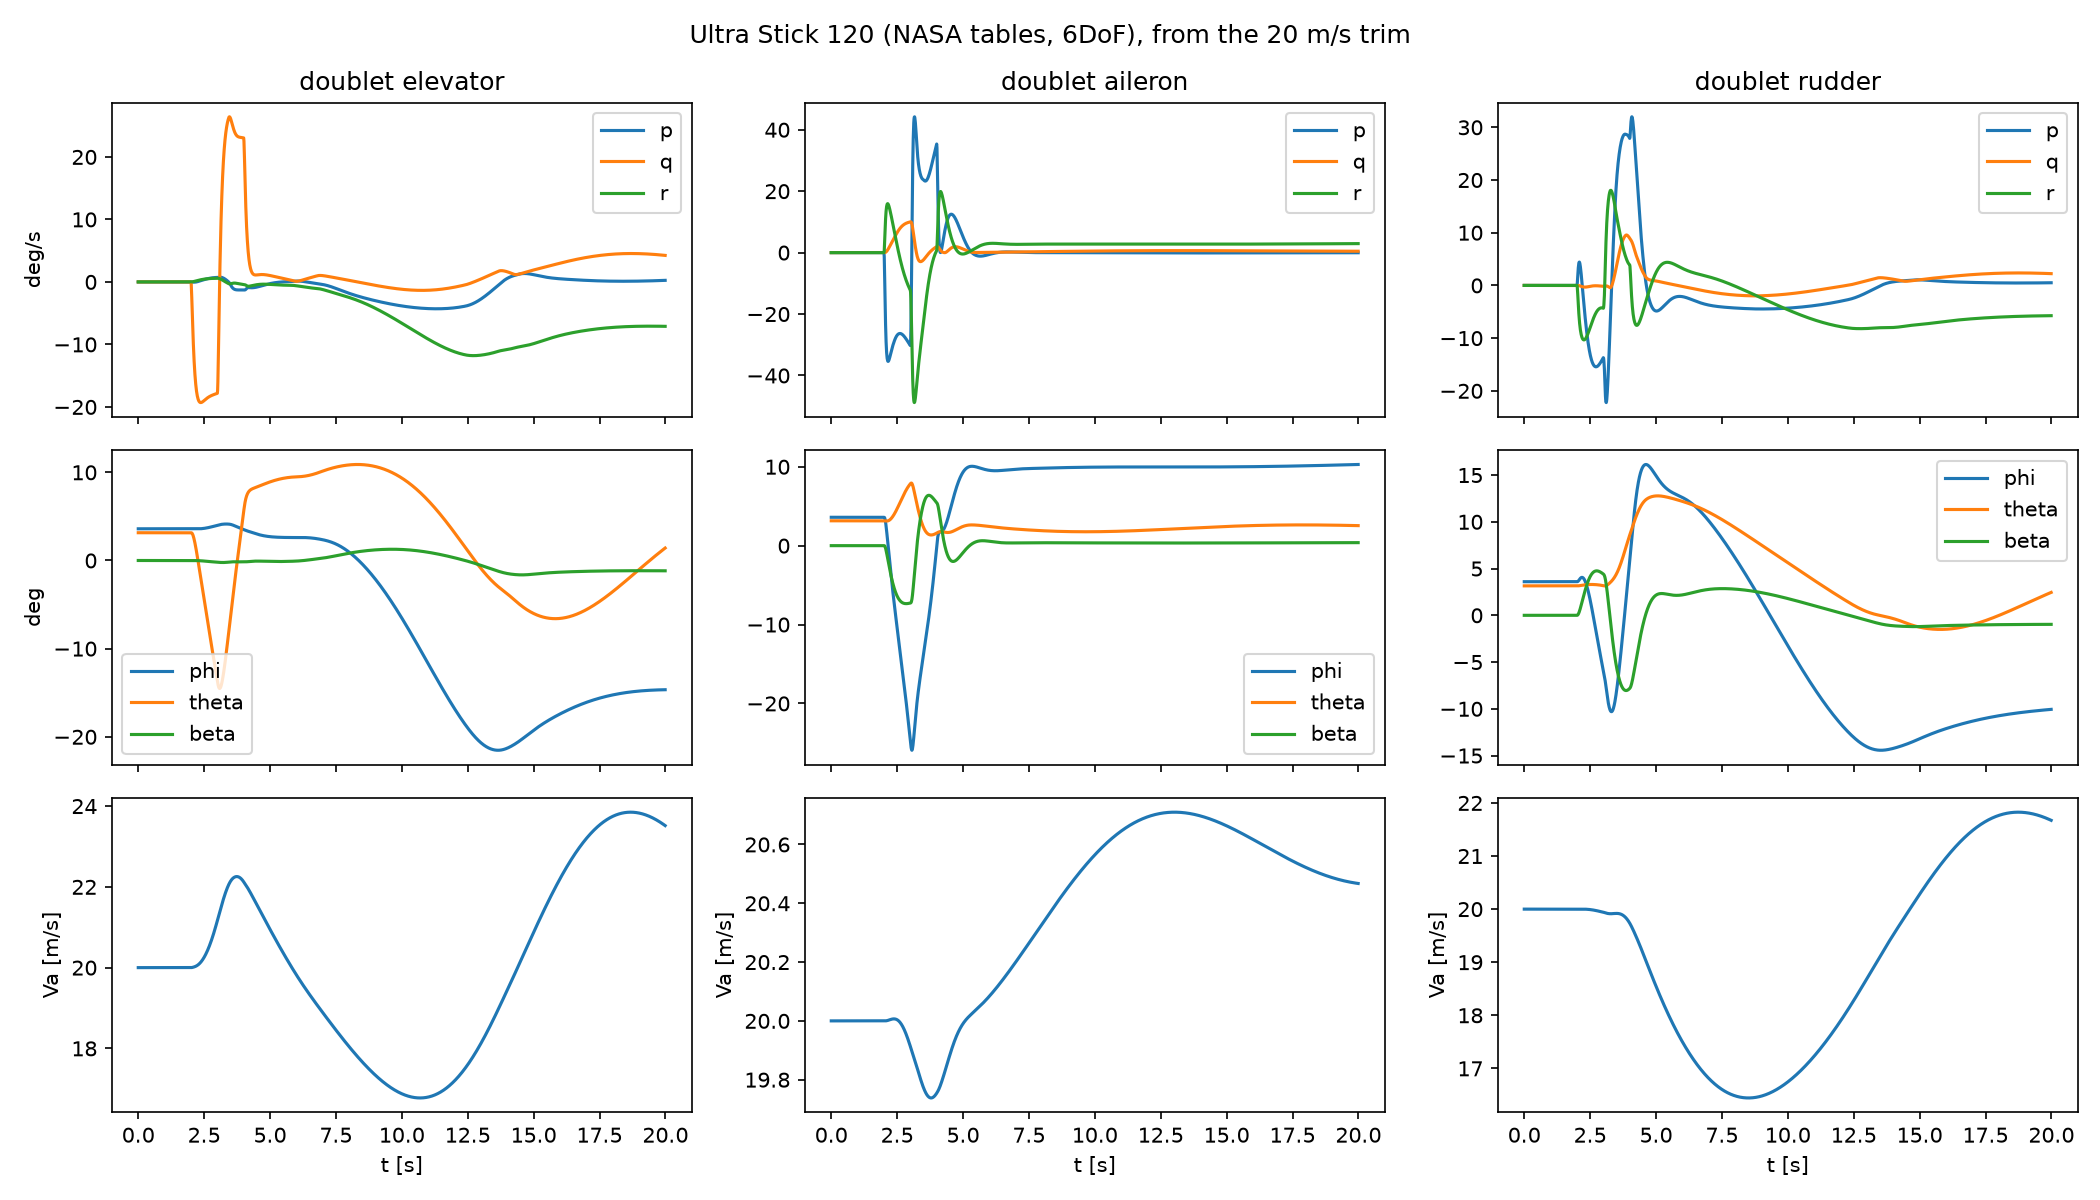
\includegraphics[width=0.7\linewidth]{../docs/figures/validation/ultrastick120_6dof_doublets.png}\par}\vspace{0.1em}}{}%
\textbf{Data.} \textbf{2,000} training flights of 30\,s in calm air (steady wind, no turbulence or gusts)
and \textbf{200} test flights of 120\,s at 20\,Hz, flown by a TECS autopilot \cite{12} with excitation
maneuvers. Every flight has its own aircraft:\par\vspace{0.1em}
{\small
\renewcommand{\arraystretch}{1.05}
\begin{tabular*}{\linewidth}{@{}l@{\extracolsep{\fill}}cc@{}}
\toprule
\textbf{randomized} & \textbf{training} & \textbf{extreme}$^{*}$ \\
\midrule
mass & $\pm 20\,\%$ & 20--35\,\% \\
inertias & $\pm 30\,\%$ & 30--45\,\% \\
aero coefficients (6, each) & $\pm 20\,\%$ & 20--30\,\% \\
motor power & $\pm 30\,\%$ & 30--45\,\% \\
CG shift (of chord) & $\pm 3\,\%$ & 3--5\,\% \\
\bottomrule
\end{tabular*}\par
\textcolor{soft}{$^{*}$ half the test flights, all parameters at once}\par}
\begin{keybox}[jepa]
\textbf{Commands} are elevator, aileron, rudder, throttle: \textbf{not forces}.
This is the key difference with SkyJEPA.
\end{keybox}
\textbf{State}: 9 quantities (airspeed, angle of attack, sideslip, $p$, $q$, $r$, roll, pitch, vertical speed).

\textbf{Sizes as in SkyJEPA}: state TCN [8,8,16], action TCN [4,4,8], GRU 24, $z \in \mathbb{R}^{24}$,
SIGReg $\lambda = 0.02$, training horizon 20 steps; history 11 steps = 0.55\,s (SkyJEPA: 10);
the estimated wind is also an input.
\fig{architecture.pdf}{\linewidth}{3.0in}
\figcap{probe = head trained on the frozen trunk.}
\textbf{Models compared}, 10.6--11.5k parameters (MLP 10,559; latent models 10,713; physics-head models 11,542):\par\vspace{0.1em}
{\small
\renewcommand{\arraystretch}{1.06}
\begin{tabular}{@{}>{\RaggedRight\arraybackslash}p{\dimexpr\linewidth-2.75in\relax}@{\hspace{0.2in}}>{\RaggedRight\arraybackslash}p{2.55in}@{}}
\toprule
\textbf{this work} & \textbf{SkyJEPA name} \\
\midrule
\mPred & Predictive \\
\mDM{} (state loss over 1-s rollouts) & not reported \\
\mJM & JEPA + prober \\
\mJP & JEPA + PI prober (their recipe) \\
\mDFP & not tested \\
\mDPE & not tested \\
\mMLP{}: raw 0.55-s window, next state = last state + MLP \cite{7} & not tested \\
\bottomrule
\end{tabular}\par}
\vspace{0.25em}
\textbf{Physics head}: outputs force and moment coefficients, is given the true mass and inertias
(no aerodynamic prior), and integrates Newton--Euler with RK4 from the last measured state.
The MLP-head models and the \mMLP{} get no aircraft parameters.
\end{panel}
\end{minipage}%
\par\vspace{\gapV}
\usebox{\refsbox}
\end{minipage}%
\hfill
\setlength{\curH}{\colH}%
% ---------------------------------------------------------------- column 3
\begin{minipage}[t][\colH][t]{\cw}\vspace{0pt}
\sbox{\colabove}{\begin{minipage}{\cw}
\begin{panel}{4}{Q1, open loop: SkyJEPA's ranking holds, the missing controls win}
\fig{fig_openloop.pdf}{\linewidth}{4.1in}
\begin{itemize}
  \item Training-range aircraft, 5\,s, 3 seeds: we reproduce SkyJEPA's ranking. \mJP{} \textbf{8.1\,m}
        beats \mJM{} \textbf{15.4\,m}, \mDFP{} \textbf{10.8\,m} and \mPred{} \textbf{37.5\,m}.
  \item The two controls SkyJEPA did not run do better: \mDPE{} \textbf{5.8\,m}, \mMLP{} \textbf{6.0\,m}.
  \item Extreme aircraft: \mJP{} is the worst, \textbf{23.6\,m} (\mJM{} 18.5, \mMLP{} 12.5,
        \mDPE{} 12.7).
\end{itemize}
\end{panel}
\end{minipage}}%
\fillrest
\begin{panel}[height=\restH]{5}{Q2, identification: the JEPA latent drops the aircraft}
\fig{fig_probe.pdf}{\linewidth}{3.95in}
$R^2$ of an MLP reader per aircraft parameter (learned representations on extreme aircraft,
raw window on training-range aircraft).
\begin{itemize}
  \item The raw 0.55-s window (states + commands) holds the motor (\textbf{0.65}) and the CG (\textbf{0.89}).
  \item \mDM{} recovers them after one GRU step (\textbf{0.49} / \textbf{0.75}).
  \item \Jep{JEPA} does not (\textbf{0.09} / \textbf{0.30}), even when its encoder also reads the commands
        (\textbf{0.14} / \textbf{0.33}, before the GRU), or with a free context latent $c$ that is not a
        prediction target (\textbf{0.13} / \textbf{0.18} vs \textbf{0.58} / \textbf{0.88} for the
        \Dir{Direct} trunk with $c$).
  \item Mass and $C_L$ are read by both (about 0.5).
\end{itemize}
\begin{keybox}[jepa]
\textbf{Why.} In a JEPA the GRU memory is the latent itself, and the loss pins $\hat z_{t+k}$ to the
encoding of a state window, which holds almost no motor or CG information (${R^2 \approx 0}$).
Why the free latent stays poor is open; one hypothesis: the objective favors slow, easy-to-predict content.
\end{keybox}
\textbf{Consequence.} A frozen \Dir{Direct} trunk + \Phy{physics head} matched end-to-end training only
with a free context latent (training range / extreme):\par\vspace{0.05em}
{\small\begin{tabular*}{\linewidth}{@{}l@{\extracolsep{\fill}}r@{}}
\Dir{Direct trunk + context, frozen,} \Phy{+ physics}, seed 0 & \textbf{6.0} / \textbf{11.1\,m} \\
\mDPE, seed 0 & \textbf{5.9} / \textbf{12.2\,m} \\
\mDFP, no context, 3 seeds & \textbf{10.8} / \textbf{16.7\,m} \\
\Jep{JEPA trunk + context, frozen,} \Phy{+ physics}, seed 0 & \textbf{8.0} / \textbf{20.6\,m} \\
\end{tabular*}\par}
\end{panel}
\end{minipage}%
\hfill
% ---------------------------------------------------------------- column 4
\begin{minipage}[t][\colH][t]{\cw}\vspace{0pt}
\begin{panel}[height=\colH]{6}{Q3, noise at equal (clean) training: JEPA acts like a low-pass filter (interpretation)}
\fig{fig_noise_openloop.pdf}{\linewidth}{3.85in}
\textbf{Open loop} (training-range aircraft, mean of seeds): \mJM{} starts high (\textbf{0.23} vs
\textbf{0.045} for the \mMLP{} at $\sigma = 0$) and grows less in relative terms ($\times 2.5$ vs
$\times 10$ at $\sigma = 0.5$); it stays above the \mMLP{} at every $\sigma$.
\fig{fig_closedloop.pdf}{\linewidth}{6.0in}
\textbf{Closed loop} (MPPI, 200 aircraft, environment seed never used for tuning, models trained on clean
data, one training seed each; tracking over the aircraft every controller kept):
\begin{itemize}
  \item \mJP{} tracks airspeed \textbf{3--9\,\%} better than \mDPE{} and the \mMLP{} under the four
        sensor-noise kinds. Gaussian 0.5: \textbf{1.19} vs \textbf{1.24} and \textbf{1.25\,m/s}
        (paired bootstrap 95\,\% CI excludes 0, 177 common aircraft); Gaussian 1.0: \textbf{1.67} vs
        \textbf{1.74} and \textbf{1.77}.
  \item Altitude tracking is mixed (\mMLP{} better under Gaussian 0.5: 7.69 vs 7.91\,m).
  \item Worse than \mDPE{} under real motion and data gaps: severe turbulence \textbf{1.49} vs
        \textbf{1.37\,m/s} (\mMLP{} 1.63); dropout 0.3: \textbf{1.05} vs \textbf{0.97}.
\end{itemize}
Smoothing would help when the fast content is fake motion and hurt when it is real. This is consistent
with JEPA favoring predictable, low-noise features \cite{5}, but we did not test it directly.
\begin{progbox}
\textbf{In progress: equal \emph{noise} training.} A denoising \Jep{JEPA} vs \mDPE{} and the \mMLP{},
trained with the same noise, tested on noise kinds never seen in training. Already measured: the
\mMLP{} trained with noise tracks at \textbf{1.20\,m/s} under Gaussian 1.0 (\mJP{}, clean:
\textbf{1.67}), but 1.62 vs 1.56\,m/s for the clean \mMLP{} under severe turbulence (separate run, its own turbulence draw).
\end{progbox}
\end{panel}
\end{minipage}%
\hfill
% ---------------------------------------------------------------- column 5
\begin{minipage}[t][\colH][t]{\cw}\vspace{0pt}
\sbox{\colabove}{\begin{minipage}{\cw}
\begin{panel}{7}{Q4, closed loop: the Plain MLP and every physics-head model fly}
\fig{fig_survival.pdf}{\linewidth}{4.0in}
\figcap{Survivors out of 200; -- = not run. Gauss.\ = Gaussian, col.\ = colored, drop.\ = dropout,
turb.\ = turbulence.}
\begin{itemize}
  \item \mTECS, the \mMLP{} and every \Phy{physics-head} model keep \textbf{199--200 of 200} aircraft
        in every condition they flew (7 conditions; the context variants 5).
  \item \mDM{} (flown in 2 conditions) loses aircraft: \textbf{177/200} under Gaussian 0.5
        (\mbox{McNemar} $p < 0.001$), \textbf{197/200} under dropout. \mJM{} was not flown here;
        it crashed every aircraft in an earlier 40-aircraft test.
  \item With the best model (\mJP), MPPI tracks airspeed \textbf{32\,\%} better than \mTECS{} under
        Gaussian 0.5 (\textbf{1.19} vs \textbf{1.75\,m/s}); \mTECS{} has no sensor filter and tracks roll better.
\end{itemize}
Survival does not separate the \mMLP{} and the physics-head models; tracking does.
\end{panel}
\end{minipage}}%
\fillrest
\begin{panel}[height=\restH]{8}{Conclusions}
\fontsize{27}{33}\selectfont
\begin{enumerate}[leftmargin=1.2em,label=\textbf{\arabic*.},itemsep=0.3em]
  \item SkyJEPA's ranking reproduces on training-range aircraft, but the \Phy{physics head} trained end to
        end (\textbf{5.8\,m}) and a \mMLP{} (\textbf{6.0\,m}) beat \mJP{} (\textbf{8.1\,m}), and \mJP{}
        is the worst on extreme aircraft.
  \item Here the commands are not forces, so the model must identify the airframe; the \Jep{JEPA} latent
        keeps little motor and CG information ($R^2$ \textbf{0.09} / \textbf{0.30} vs \textbf{0.49} /
        \textbf{0.75}), even with a free context latent.
  \item At clean training, the \Jep{JEPA} trunk tracks \textbf{3--9\,\%} better under sensor noise and worse
        than the end-to-end physics model under turbulence: it smooths.
  \item With 9 states, a \mMLP{} of 10.6k parameters on the raw window predicts as well as the best
        physics model and better than the JEPA models.
\end{enumerate}
\begin{keybox}[phys]
\textbf{Where JEPA could still help}: rich observations with distractor channels or images (next step).
\end{keybox}
\begin{keybox}[soft]
\textbf{Limits}: simulation only; one airframe family; one training seed per model in closed loop;
physics heads receive the true mass and inertia, the other models do not; the link to
``commands are not forces'' is not tested by varying the command type.
\end{keybox}
\end{panel}
\end{minipage}

\end{document}
